\chapter{Combat}\label{Combat}
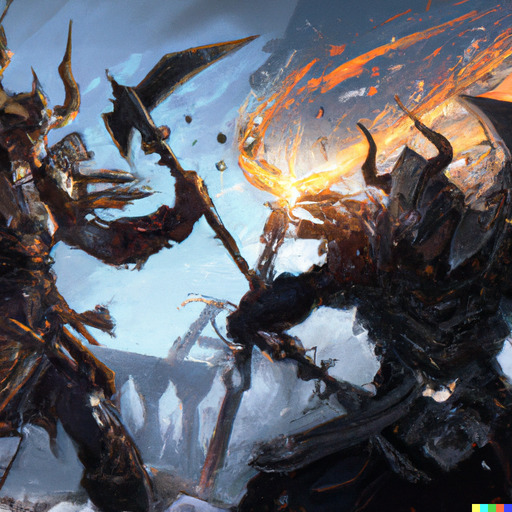
\includegraphics[width=\columnwidth]{combat/combat}

The world of Rise can be a harsh one, and not all disagreements can be resolved peacefully.
At some point, you will be forced to enter combat.
This chapter explains how combat works in Rise.
The combat rules also generally cover situations where time and precise positioning are important, even if they do not involve violence.

\section{Attacking and Defending}
  When you use an offensive ability, you will have to make an attack.
  To make an attack, roll 1d10 and add your \glossterm{accuracy} with the attack.
  That should be written on your character sheet in the attack's description.
  If you get a 10, keep rolling until you don't, then sum all of the rolls.

  Your attack result is compared to your target's relevant defense.
  There are four defenses: Armor, Fortitude, Reflex, and Mental.
  Each attack specifies what defense the target uses to avoid the attack.

  There are four possible outcomes for an attack: a critical hit, a regular hit, a glancing blow, and a miss.
  \begin{itemize}
    \item Critical hit: Your attack result exceeds the target's defense by at least 10.
      A critical hit deals double damage, and may have other special effects.
    \item Hit: Your attack result meets or exceeds the target's defense.
      The ability has its normal effect.
    \item Glancing blow: Your attack result was too low, but only 1 or 2.
      The ability deals half damage, and doesn't have any special effects other than damage.
    \item Miss: Your attack was too low by 3 or more.
      The ability has no effect unless it specifically says it does.
  \end{itemize}

  This process works in the same way when enemies attack you.
  The GM may ask you what your defenses are when attacking you.

\section{Dealing and Taking Damage}
  If you hit with a damaging attack, you roll the damage dice for that attack, sum them all together, and tell the GM the result.
  Many abilities also add a flat amount to the damage result.
  The GM will track that damage and tell you what effect it had.

  Taking damage is more complicated.
  When you take damage, the damage first reduces your \glossterm{damage resistance}.
  Any damage in excess of your remaining damage resistance causes you to lose that many \glossterm{hit points}.
  Hit points and damage resistance function in the same way, but damage resistance can protect you from debilitating attacks that only work if they make you lose hit points.
  If you are dealt damage that reduces your hit points below 0, you gain one or more \glossterm{vital wounds}.

  While you have vital wounds, you suffer penalties based on the wound.
  If you get more than one vital wound, you can die.
  The GM can explain how vital wounds work in more detail if it comes up.
  Vital wounds can only be removed with an 8 hour rest, or with some rare abilities which you probably won't have access to.

\section{Tracking Time in Combat}
  Combat takes place in a series of \glossterm{rounds}, which represent about six seconds of time.
  Each round of a combat is divided into two \glossterm{phases}: the movement phase and the action phase (see \pcref{Phases}).
  After both phases are complete, the round ends and the next round begins.

  During the movement phase, everyone will move, but can't attack.
  During the action phase, everyone will take a \glossterm{standard action} of their choice.
  This could be an attack, an additional movement, or another special ability.

  You and your fellow player characters will take turns during each phase, but you can act in any order.
  The GM might ask each player in turn what they plan to do, or players could decide for themselves what they want to do and tell the GM whenever they have decided.
  It depends how the GM wants to run the game.

  While your characters take actions, your enemies will also take their own actions.
  Their actions resolve simultaneously with your actions.
  The GM will typically tell you what your enemies did after all of the players have finished their actions.

  \subsection{Action Types}
    Most abilities require a \glossterm{standard action} to use.
    You can take one standard action during each action phase.

    Some less common abilities require a \glossterm{minor action}.
    You can take one minor action during each action phase in addition to your standard action.

    There are also \glossterm{free actions}, which aren't generally used for specific player abilities.
    You can take any number of free actions during both the movement and action phase.

\section{Movement}
  During the movement phase, your character move up to their speed along the ground.
  Most characters have a movement speed of 30 feet, but your character sheet will tell you your speed.
  You tell the GM which location you want to move to, or which creature you want to move next to.
  If you move during the action phase, you can sprint, which doubles your movement speed.
  Enemies will still get a chance to attack you from your original position even if you move during the action phase, so you can't dodge attacks that way.

  You might be playing with a gridded battlemap with figures for each character, or you might be just imagining the world.
  Movement on a grid or hex map is typically more precise and tactical, while purely mental scenes tend to be more loose about exact distances and positioning.
  As usual, talk to your GM about what you each want from the game.

\section{Universal Combat Abilities}
  Your character sheet will have some abilities unique to your character written on it.
  In addition, there are a variety of things that every character can do in the world.
  These won't generally be written on your sheet explicitly because they are the same for everyone.
  However, it can be useful to know that they exist.
  If you find yourself using one of these abilities often, consider adding it to your character sheet.

  % Keep in sync with ToC/Combat.tex
  \begin{itemize}
    \item Charge: Move and make a strike with a weapon, but suffer a brief \minus2 penalty to defenses afterwards.
    \item Desperate Exertion: Reroll any attack or check with a \plus2 bonus, but you gain two \glossterm{fatigue levels}.
    \item Escape Grapple: Stop being grappled.
    \item Grapple: Start grappling with a foe.
    \item Maintain Grapple: Continue grappling with a foe as a \glossterm{free action}.
    \item Overrun: Move through spaces occupied by enemies. Costs one fatigue during the movement phase, but is free during the action phase.
    \item Recover: Regain half your hit points, all your damage resistance, and remove all conditions. However, you gain two fatigue levels, and you can only do it once per fight.
    \item Shove: Push a foe up to half your speed.
    \item Sprint: Move at double speed. Costs one fatigue during the movement phase, but is free during the action phase.
    \item Total Defense: Gain a \plus2 bonus to all defenses this round.
    \item Throw: Throw something you're holding.
    \item Trip: Knock a foe \prone.
  \end{itemize}

\section{Using Abilities}\label{Using Abilities}
  % TODO: narrative text explaining how you talk about using abilities as a player.

  \subsection{Ability Descriptions}
    Abilities are typically written in the following form:
    \begin{activeability}{Ability Name}[Ability Tags (if any)]
      \abilityusagetime Usually a standard action
      \rankline
      This section will explain who or what the ability affects, and how those targets are affected.
      Many abilities cause you to make an attack.
      \hit This describes the effect that the ability has against a target that you successfully hit with it.
      \crit If the ability has a special effect on a \glossterm{critical hit}, that effect is described here.
      \miss Some abilities still deal half damage even when they miss.
    \end{activeability}

  \subsection{Magical and Mundane Abilities}\label{Magical and Mundane Abilities}
    Every ability is either \magical or mundane.
    Magical abilities use Willpower to determine their \glossterm{power}, while mundane abilities use Strength.
    If an ability has a \sparkle{} next to its name, it is magical.
    Otherwise, it is mundane.

  \subsection{Ability Range}\label{Ability Range}
    Many abilities only work within a particular distance from you.
    This maximum distance is called the ability's \glossterm{range}.
    There are five common ranges: \shortrange, \medrange, \longrange, \distrange, and \extrange.

  \subsubsection{Line of Sight}
    You have \glossterm{line of sight} to something if you can see it.
    Glass does not block line of sight, but darkness and fog can.

  \subsubsection{Line of Effect}
    You have \glossterm{line of effect} to something if you could touch it with a really long pole.
    Glass blocks line of effect, but darkness and fog do not.

  \subsection{Targeted Abilities}\label{Targeted Abilities}
    If an ability affects a specific number of creatures or objects, it is called a \glossterm{targeted} ability.
    Targeted abilities require you to have \glossterm{line of sight} and \glossterm{line of effect} to all targets.
    Every targeted ability has a \glossterm{range}.

  \subsection{Area Abilities}\label{Area Abilities}
    If an ability affects everything of a certain type within an area, it is called an area ability.

    % TODO: should emanation be its own unique category?
    % An emanation is always a radius, does not have a single point of origin, etc.
    \subsubsection{Area Types}
      There are three common area types.
      If an area's type is not mentioned, it is a burst.
      \begin{raggeditemize}
        \item Burst: Has an immediate effect and then ends.
        \item Emanation: Has a duration based on a specific creature or object. If the source of the area moves, the area's effect moves with it.
        \item Zone: Has a duration based on a location. Some zones can be moved after being created, but that movement is not tied to a specific creature or object.
      \end{raggeditemize}

    \subsubsection{Measuring Areas}
      Areas are always measured from a \glossterm{point of origin}, which must be a grid intersection.
      An area's size defines the extent to which it extends out from its point of origin, whether as a radius or as a length.
      All four of a square's corners must be within an area for that square to be in the area.

      When using an area ability, you must have \glossterm{line of sight} and \glossterm{line of effect} to its point of origin.
      The ability's \glossterm{range} measures the maximum distance to its point of origin.
      If it does not have a range, its point of origin must touch your space.

      There are six common area sizes: \tinyarea, \smallarea, \medarea, \largearea, \hugearea, and \gargarea.

      There are five common area shapes.
      If an area's shape is not mentioned, it is a sphere.
      \begin{raggeditemize}
        % TODO: cones don't make sense with a single point of origin. Add pictures?
        \item Cone: A 90 degree arc, measured by length. A cone's height is normally 5 feet.
        \item Cylinder: A circle with a height, measured by radius. A cylinder's height is normally equal to its radius.
        \item Line: A straight line, measured by length. A line is normally 5 feet wide and 5 feet high.
        \item Sphere: A sphere, measured by radius.
        \item Wall: A straight line, measured by length. A wall's height is normally equal to half its length, and its width is essentially zero. A wall is always a \glossterm{zone}, not a \glossterm{burst} or an \glossterm{emanation}.
      \end{raggeditemize}

  \subsection{Dismissal}\label{Dismissal}
    When an ability is \glossterm{dismissed}, all of its lingering effects immediately end.
    Unless otherwise noted, all \magical abilities with a duration can be dismissed, but \glossterm{mundane} abilities cannot be dismissed.
    % Seems unnecessary
    % This includes \glossterm{conditions}, \glossterm{brief} effects, and other abilities with more specific durations.
    You can dismiss abilities as a \glossterm{free action} that requires only mental effort.
